\documentclass[11pt,a4paper]{ctexart}
\usepackage[margin=2.3cm]{geometry}
\usepackage{amsmath,amssymb,bm}
\usepackage{booktabs}
\usepackage{graphicx}
\usepackage{xcolor}
\usepackage{caption}
\usepackage{enumitem}
\usepackage[colorlinks=true,linkcolor=blue!50!black,urlcolor=blue!50!black]{hyperref}
\setCJKmainfont{Noto Sans CJK SC}
\setCJKsansfont{Noto Sans CJK SC}
\captionsetup{font=small}
\renewcommand{\arraystretch}{1.12}
\setlist[itemize]{leftmargin=1.4em,itemsep=0.15em,topsep=0.25em}
\setlist[enumerate]{leftmargin=1.5em,itemsep=0.15em,topsep=0.25em}

\title{\bfseries 双 MCT 猫道扭转偏差：讨论整理\\
\large 从表 4--1 差异、理论修复、图纸核证到 $f99$ 全模型路径}
\author{讨论整理稿（Fable / 双 MCT 复算）}
\date{2026 年 8 月 27 日}

\begin{document}
\maketitle

\noindent\fbox{\parbox{\dimexpr\linewidth-2\fboxsep}{
\textbf{性质声明（not\_a\_scientific\_claim）}：本文是把此前讨论整理成一份可独立阅读的记录，不是新的科学结论。全部频率均取自仓库已锁证据或已提交复算；不重跑求解器、不拟合、不宣布复现附件。附件 2--3 表 4--1 只作对照，不参与任何模型构建。
}}

\tableofcontents
\vspace{0.6em}

\section{这份整理写什么}

此前讨论按时间顺序走了五步：
\begin{enumerate}
  \item 只分析：附件 2--3 表 4--1 与双 MCT（门架素正后）正式配对差在哪里；
  \item 诊断：MCT 简化模型的扭转通路缺了什么；
  \item 理论推导修复：双索组、双簇端口、质量空间化，并给出推导 PDF；
  \item 图纸核证：U 栓 / 尼龙滚轮 / 销 / 抱箍，以及 drawing-soft 变体；
  \item 对照另一条路径：\texttt{f99-chain-closure} 上的全尺度 ANSYS 链（S10$\to$C20$\to$D10$\to$E10$\to$E20）。
\end{enumerate}
用户原句是``把以上讨论整理成 PDF 发给我''。本文把五步收成一份叙事：先给数字，再给机制，最后给能说 / 不能说的边界。更细的公式与复现命令见同目录推导稿
\texttt{double\_mct\_torsion\_theory\_fix\_cn.pdf}。

\section{起点：表 4--1 与双 MCT 正式配对}

锁定证据来自
\texttt{modal\_validation/gate\_corrected\_reference\_table4\_1\_matching.csv}
与 \texttt{gate\_corrected\_findings.md}。配对规则与锁定版同层级：主跨能量 $\ge0.65$ + 家族 + 奇偶性 + 家族内升频序号；半波 MAC 只作指纹，不把 TS2 改配到 TS3。

\begin{table}[h]\centering\footnotesize
\begin{tabular}{llrrrr}
\toprule
行 & 描述 & 附件 Hz & 旧配对 Hz & 误差 & 族 \\
\midrule
LS1 & 一阶正对称横弯 & 0.0365 & 0.036773 & $+0.75\%$ & 非 T \\
VA1 & 一阶反对称竖弯 & 0.0700 & 0.071446 & $+2.07\%$ & 非 T \\
LA1 & 一阶反对称横弯 & 0.0726 & 0.073502 & $+1.24\%$ & 非 T \\
TA1 & 一阶反对称扭转 & 0.0996 & 0.071491 & $\bm{-28.22\%}$ & T \\
VS1 & 一阶正对称竖弯 & 0.1028 & 0.101177 & $-1.58\%$ & 非 T \\
LS2 & 二阶正对称横弯 & 0.1087 & 0.110112 & $+1.30\%$ & 非 T \\
TS1 & 一阶正对称扭转 & 0.1147 & 0.100981 & $\bm{-11.96\%}$ & T \\
SIDE1 & 边跨 & 0.1149 & 0.116182 & $+1.12\%$ & 非 T \\
SIDE2 & 边跨 & 0.1239 & 0.124815 & $+0.74\%$ & 非 T \\
VA2 & 二阶反对称竖弯 & 0.1438 & 0.146445 & $+1.84\%$ & 非 T \\
LA2 & 二阶反对称横弯 & 0.1449 & 0.146579 & $+1.16\%$ & 非 T \\
SIDE3 & 边跨 & 0.1557 & 0.164799 & $+5.84\%$ & 非 T \\
TS2 & 二阶正对称扭转 & 0.1571 & 0.143814 & $\bm{-8.46\%}$ & T \\
VS2 & 二阶正对称竖弯 & 0.1744 & 0.145334 & $-16.67\%$ & 非 T$^\ast$ \\
\midrule
\multicolumn{4}{l}{14 行 MAE / RMS} & $5.92\%/9.78\%$ & \\
\multicolumn{4}{l}{T 族 / 非 T MAE} & $16.21\%/3.12\%$ & \\
\bottomrule
\end{tabular}
\caption{锁定正式配对。$^\ast$VS2 名义上非 T，但误差量级与 T 族同档，后文单独处理。}
\end{table}

\begin{figure}[h]\centering
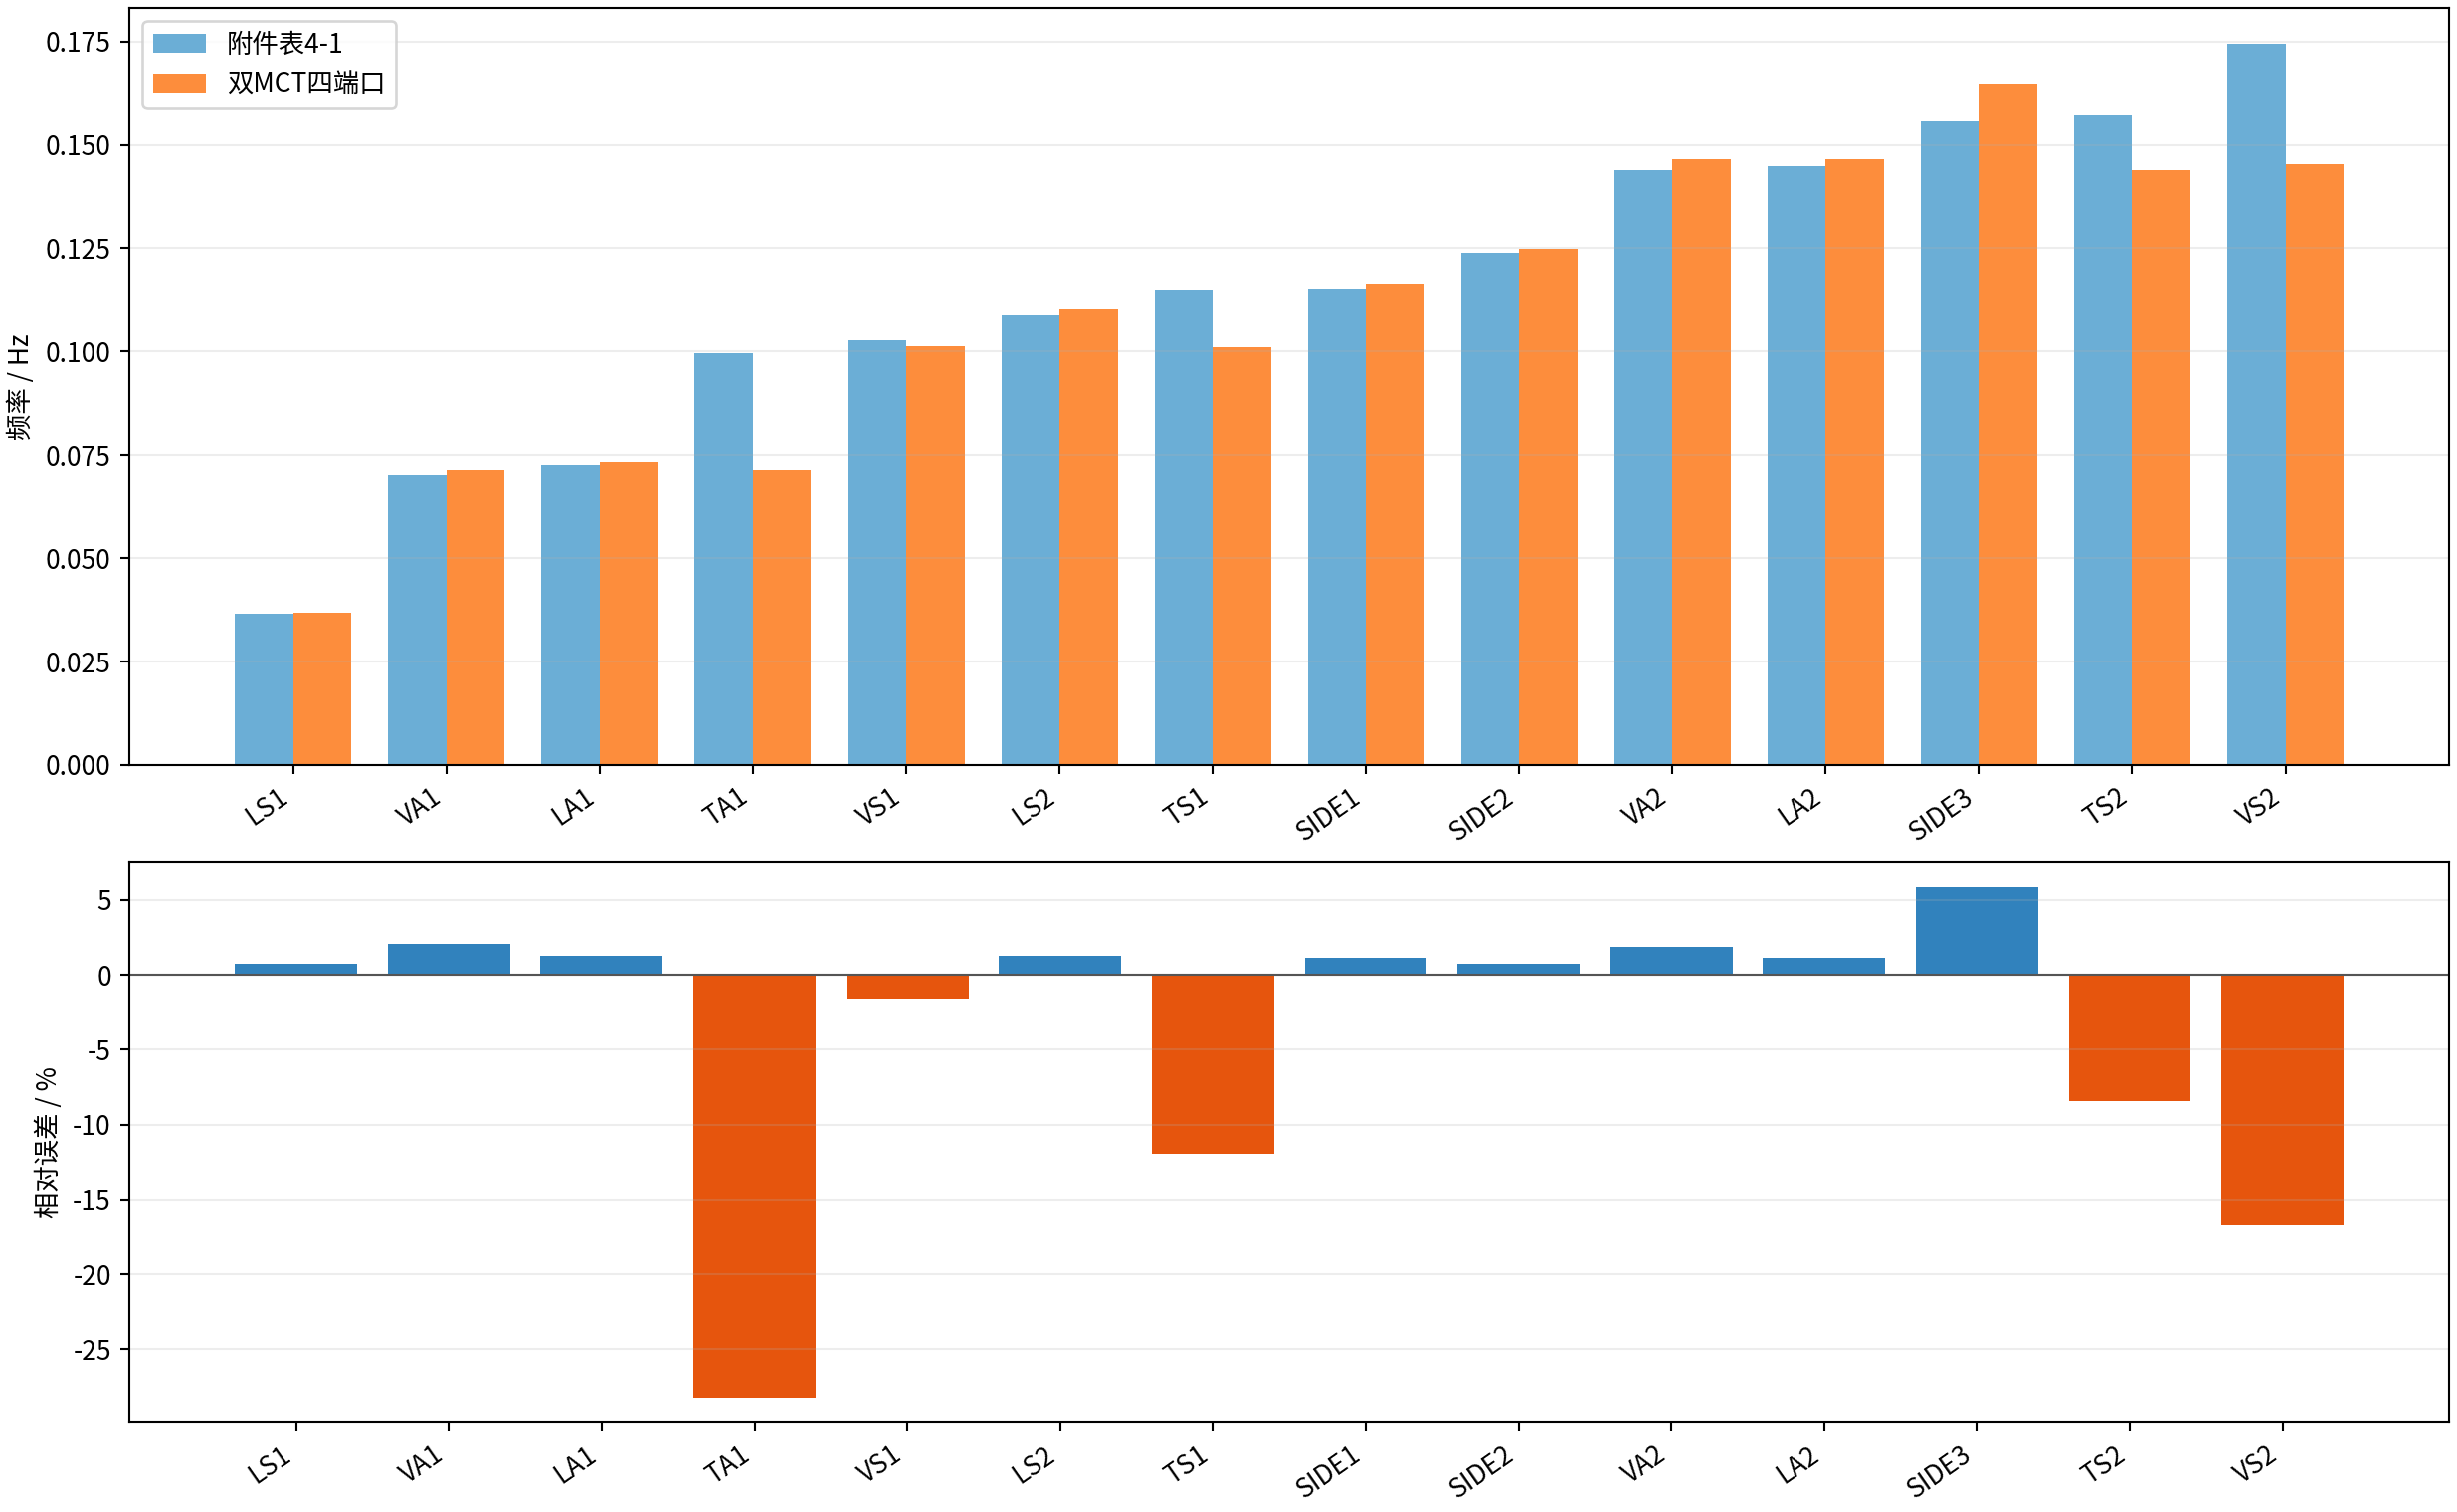
\includegraphics[width=0.96\linewidth]{assets/modal_14_mode_validation.png}
\caption{当时交付包里的十四行对照：L/V 主跨贴附件，T 族与 VS2 系统性偏低。}
\end{figure}

\textbf{当时能说}：非 T 主跨行（LS/LA/VA/VS1）在 $\pm2\%$ 内；偏差集中在 T 三行，且 TA1 几乎正好落在 VA1 上（分裂 $0.063\%$）。
\textbf{当时不能说}：不能把半波 MAC 当正式配对依据；不能宣布``T 族算错了所以附件对''或反过来。

\section{当时的诊断：MCT 模型哪里有问题}

旧正式 ROM 把每幅压成零宽平面。模型里叫``T 族''的东西，运动学上是两幅差分竖向，与 V 族近简并。附件却要求 TA1/TS1/TS2 相对对应竖弯分离 $+42.3\%/+11.6\%/-9.9\%$。T 族误差几乎恰好等于``扭转塌缩到竖弯''的差值。

三条被平面化切断的通路：
\begin{itemize}
  \item 幅内滚转自由度与滚转惯量（平面模型 $J_\varphi=0$）；
  \item 门架横向框架作用（秩一轴杆后为零；原先的固定转角横剪上界 $80.7$~N/mm 被判定为非客观）；
  \item 横通道滚转传递（单中心平动端口凝聚后滚转不可观，T 模态里 K12 应变能 $\le0.34\%$）。
\end{itemize}
当时的合理假设是：把这三条通路按审计部件客观补回去，T 族就会离开竖弯、靠近附件。后面的推导就是在验证这个假设。

\section{理论修复做了什么}

全部参数取自仓库审计数据，无拟合旋钮。三项结构修复：

\paragraph{双索组等效}
每幅承重索束按 16 根 $\phi50$ 实索偏距的均方根拆为 $\pm b_B$（$b_B=1.858$~m），门架索束按 6 根 $\phi54$ 拆为 $\pm b_T$（$b_T=1.962$~m）。共模（同相）动力学严格不变；幅内滚转的几何刚度 $\sum T_i y_i^2$ 与惯量 $\sum m_i y_i^2$ 按实索排布精确恢复。

\paragraph{双簇端口凝聚}
否决了``保留转角 + 刚性截面伪逆展开''（它把 5.34~m 幅宽锁成平板，Rayleigh 把滚转推到 $1.5$--$3.8$~Hz）。改用每接口两个索簇平动子端口、转角全部自由凝聚：门架 $12\times12$ 恰 6 个刚体零模 + 6 个正弹簧；横通道 $24\times24$ 恰 6 个刚体零模 + 18 个正弹簧。滚转可观，簇间横梁柔性保留。转角自由凝聚对应``索不向门架传弯矩''——这是 U 栓抱夹的物理事实，不是简化。

\paragraph{二期质量空间化}
963.811~t 二期质量按质量空间化审计 V2.0 的 33003 个真实坐标分配，保 0/1 阶矩；总质量闭合误差 $9.7\times10^{-10}$~t。

实现：$4500$ 节点、$13500$ 平动自由度，80 阶 shift-invert。特征对残差 $\le4.9\times10^{-10}$。与锁定旧模型前 24 阶质量加权 MAC $0.94$--$0.99994$，主跨行频移 $\le1.1\%$——升级是受控细化，不是模型漂移。两类非物理分支被治愈：双索组``呼吸''机构消失；旧 M37 起 13 阶门架索横向解耦分支转为受约束的系统横向分支。

\section{修复后的数字：T 族几乎不动}

\begin{table}[h]\centering\footnotesize
\begin{tabular}{lrrrrrr}
\toprule
行 & 附件 & 旧 Hz & 旧误差 & 升级 Hz & 升级误差 & drawing-soft \\
\midrule
LS1 & 0.0365 & 0.036773 & $+0.75\%$ & 0.036825 & $+0.89\%$ & $+0.88\%$ \\
VA1 & 0.0700 & 0.071446 & $+2.07\%$ & 0.071142 & $+1.63\%$ & $+1.63\%$ \\
LA1 & 0.0726 & 0.073502 & $+1.24\%$ & 0.073147 & $+0.75\%$ & $+0.73\%$ \\
TA1 & 0.0996 & 0.071491 & $-28.22\%$ & 0.071093 & $\bm{-28.62\%}$ & $\bm{-28.66\%}$ \\
VS1 & 0.1028 & 0.101177 & $-1.58\%$ & 0.101626 & $-1.14\%$ & $-1.14\%$ \\
LS2 & 0.1087 & 0.110112 & $+1.30\%$ & 0.109799 & $+1.01\%$ & $+0.95\%$ \\
TS1 & 0.1147 & 0.100981 & $-11.96\%$ & 0.101135 & $\bm{-11.83\%}$ & $\bm{-11.86\%}$ \\
SIDE1 & 0.1149 & 0.116182 & $+1.12\%$ & 0.120952 & $+5.27\%$ & $+5.22\%$ \\
SIDE2 & 0.1239 & 0.124815 & $+0.74\%$ & 0.125595 & $+1.37\%$ & $+1.35\%$ \\
VA2 & 0.1438 & 0.146445 & $+1.84\%$ & 0.146060 & $+1.57\%$ & $+1.57\%$ \\
LA2 & 0.1449 & 0.146579 & $+1.16\%$ & 0.144864 & $-0.02\%$ & $-0.17\%$ \\
SIDE3 & 0.1557 & 0.164799 & $+5.84\%$ & 0.165908 & $+6.56\%$ & $+6.45\%$ \\
TS2 & 0.1571 & 0.143814 & $-8.46\%$ & 0.142913 & $\bm{-9.03\%}$ & $\bm{-9.15\%}$ \\
VS2 & 0.1744 & 0.145334 & $-16.67\%$ & 0.144424 & $-17.19\%$ & $-17.19\%$ \\
\midrule
T 族 MAE & & & $16.21\%$ & & $16.49\%$ & $16.56\%$ \\
非 T MAE & & & $3.12\%$ & & $3.40\%$ & $3.39\%$ \\
\bottomrule
\end{tabular}
\caption{三条结构通路全部补回之后，主跨 L/V 普遍改善或持平；T 三行漂移 $<0.7$ 个百分点。drawing-soft 见第 \ref{sec:drawings} 节。}
\end{table}

\begin{figure}[h]\centering
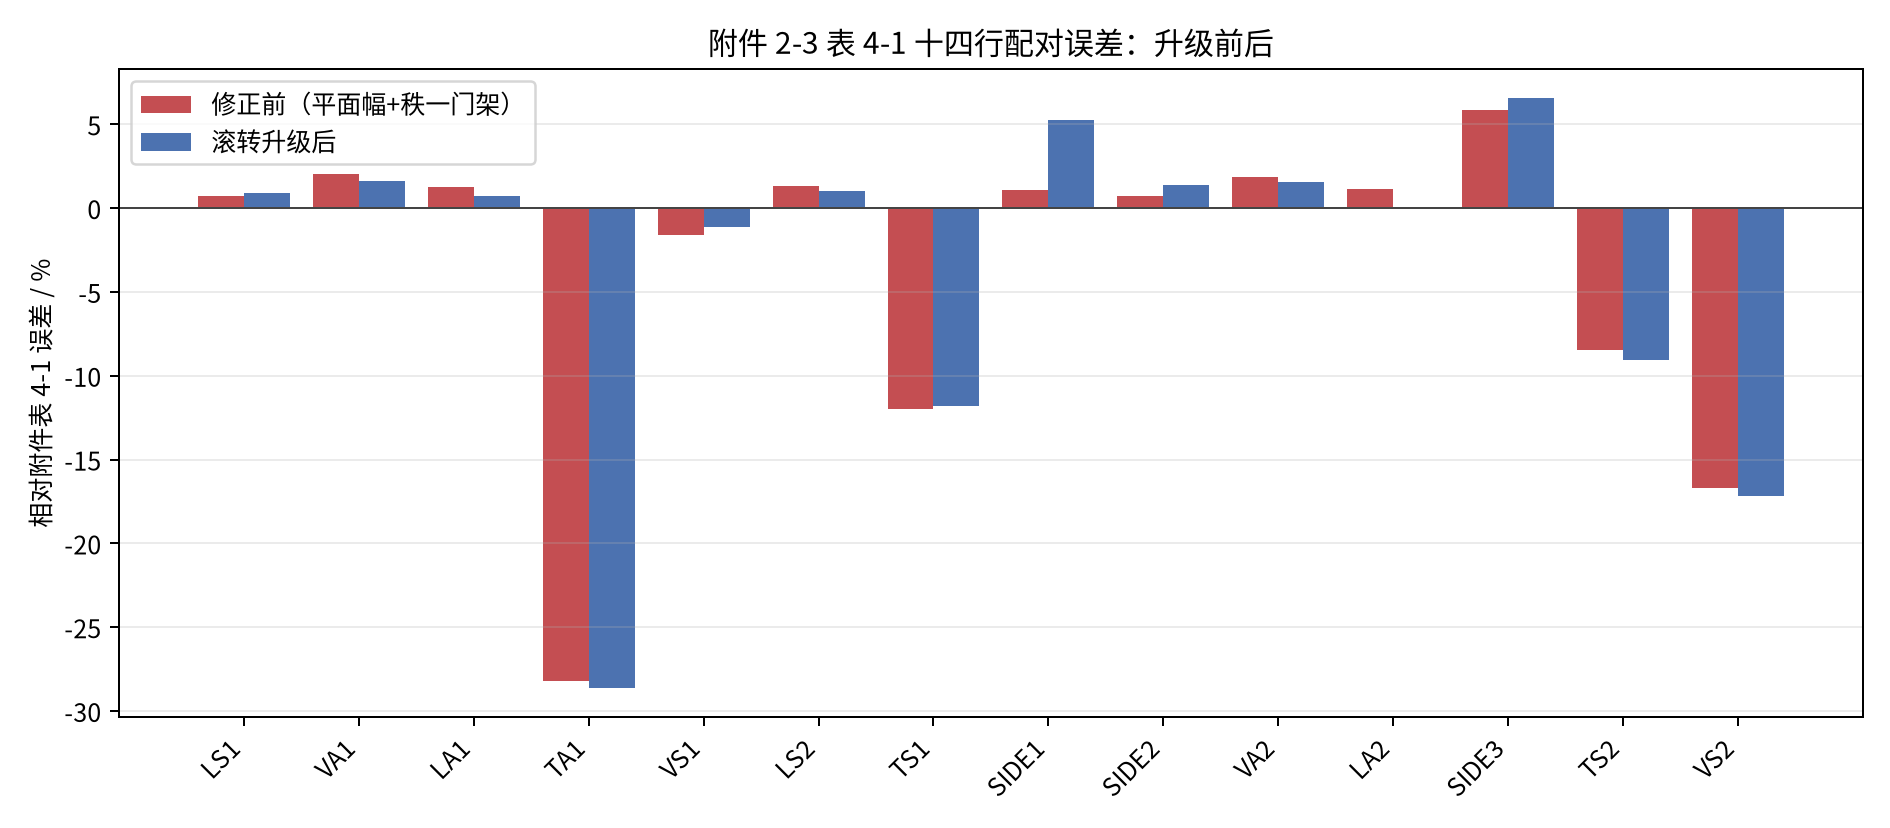
\includegraphics[width=0.98\linewidth]{../roll_upgraded_results/roll_upgraded_error_comparison.png}
\caption{升级前后十四行误差。T 三行几乎重叠——这不是实现失败，而是下一节的结构事实。}
\end{figure}

假设被证伪：补回平面化切断的三条通路，并不能把 T 族抬到附件。问题从``模型少装了刚度''变成``这些审计部件客观上到不了那个频率''。

\section{扭转可达域（括弧定理）}\label{sec:bracket}

\subsection{引理 A：系统扭转钉扎}

双幅整体扭转（刚体旋转型 $w_i=\psi(x)\,y_i$）满足
\begin{equation}
\frac{\lambda_T}{\lambda_V}
=\frac{\sum_i T_i y_i^2\big/\sum_i m_i y_i^2}{\sum_i T_i\big/\sum_i m_i}.
\end{equation}
本结构张力与质量的横向分布同构（都集中在 $\pm21.45\pm b$ 的索线上，幅间构件仅 150~t），故 $\lambda_T/\lambda_V\approx1$。数值：新模型 TA1--VA1 分裂 $0.069\%$，旧模型 $0.063\%$——两代完全不同的门架 / 横通道处理给出同一结果。反对称系统扭转无净索伸长（Irvine 项为零），弹性无法把它抬升。要使 $\lambda_T/\lambda_V=1.423^2$，质量横向 rms 必须缩到 15.1~m（现约 21.5~m），即约一半质量移到幅间——与任何审计质量数据不符。

这就是讨论里说的``摆式物理''：系统扭转被钉在竖弯族上，与连接刚度无关。后文 $f99$ 链从 S10 到 E10 的 TA1 始终停在 $0.0733$--$0.0734$~Hz（$\approx2f^\ast$ 纯张力反对称根），是同一条引理的全模型版。

\subsection{引理 B：幅内滚转锁定}

把幅内滚转场放到 Rayleigh 商上：即使换成更柔的双簇端口，滚转分支仍在 $1.0$~Hz 以上（全侧摆反相 1.05~Hz；无侧摆 2.8--3.6~Hz）。控制性刚度是审计钢结构的滚转传递：门架 $4.7\times10^{6}$--$6.9\times10^{7}$、横通道 $0.98$--$2.6\times10^{8}$~N·m/rad。它们把幅内滚转推到比附件 TA1 高一个量级的地方，进不了 0.08--0.17~Hz 窗口。

\subsection{括弧}

两条引理把可达域夹成一个括弧：
\begin{itemize}
  \item 下沿：系统扭转 $=$ 摆式地板 $\approx$ VA1 $\approx0.071$~Hz；
  \item 上沿：幅内独立滚转 $\ge1.0$~Hz，被钢结构锁死。
\end{itemize}
0.08--0.17~Hz 之间不存在由现有审计部件客观装配出来的独立扭转分支。附件 TA1$=0.0996$~Hz 正好落在这个空档里。

由附件 TA1 反推：若只靠分布滚转弹簧把系统扭转从 0.0711 抬到 0.0996，每品门架有效滚转约束约 $1.5\times10^{4}$~N·m/rad（TS1 反推 $0.9\times10^{4}$），比审计刚接低 2--4 个数量级。这是需求值，不是来源值；在取得设计出处之前把它当旋钮调到附件，等于拟合。本文不做。

\section{图纸连接：柔性端也推不动}\label{sec:drawings}

用户指出``图纸有连接方式''，并点名《图纸汇总-2026.08.05.pdf》。从 Release \texttt{zhangjinggao-full-20260729}（archive-0001）取得的是 1225 版 124 页施工图；175 页汇总版不在该归档内。与扭转通路相关的构造：

\begin{itemize}
  \item \textbf{承重索—门架}（MD1-04/05）：每根 $\phi50$ 用一副 M14 U 型螺栓抱夹于底梁——逐索点式传力，无弯矩约束，与凝聚采用的 UXYZ 一致。
  \item \textbf{门架}（MD4-01/02）：$\Box160\times160\times4$，高 8~m（可调 7.5--8.3~m，$\phi16$ 销），顶部楔块夹 6-$\phi54$ 门架承重绳。
  \item \textbf{通道—猫道}（MD5-16/17、MD5-24/25）：通道支架经 32 只 MC 尼龙滚轮 $\phi60\times50$ 骑在承重索上；竖向支撑为 $\phi34$ 销 + R76 抱箍。\textbf{通道与门架之间不存在任何刚接节点}。审计 APDL 把通道与门架焊死的 74 条 CERIG,ALL 是偏刚的理想化。
\end{itemize}

据此构造 drawing-soft 变体：50 个普通站用双簇门架，21 个通道站改回原审计平动 K12（滚转透明）。结果：T 族 $-28.66/-11.86/-9.15\%$。与刚接变体（$-28.62/-11.83/-9.03$）及锁定旧版（$-28.22/-11.96/-8.46$）对比：\textbf{横跨``图纸柔性端—审计刚接端''的全部物理连接刚度区间，T 族误差漂移小于 0.7 个百分点}。引理 A 被图纸反向加固。

\begin{figure}[h]\centering
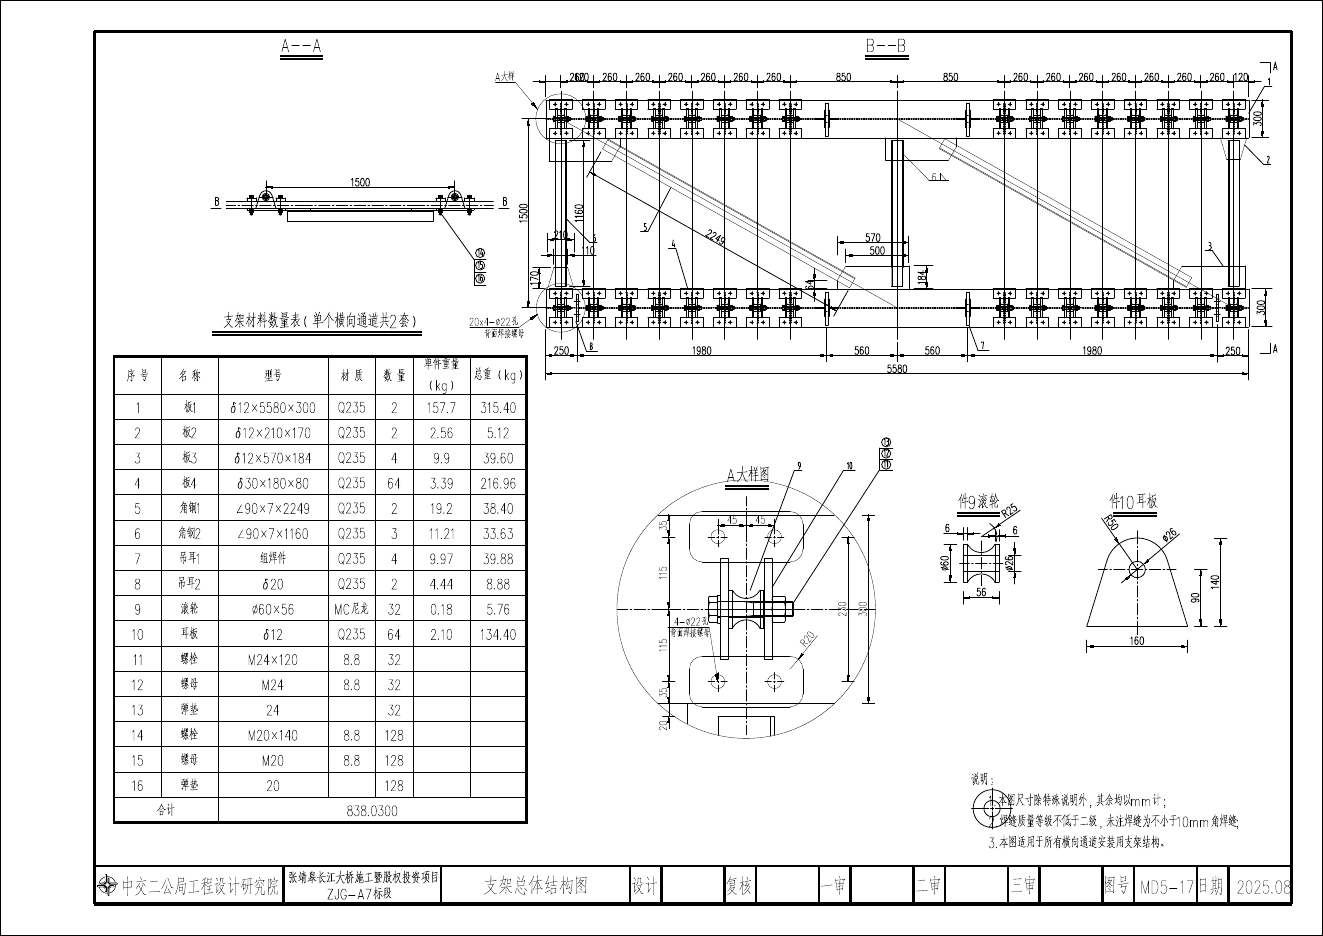
\includegraphics[width=0.48\linewidth]{../inputs/roll_upgrade_sources/drawing_evidence/MD5-17_support_nylon_rollers.png}
\hfill
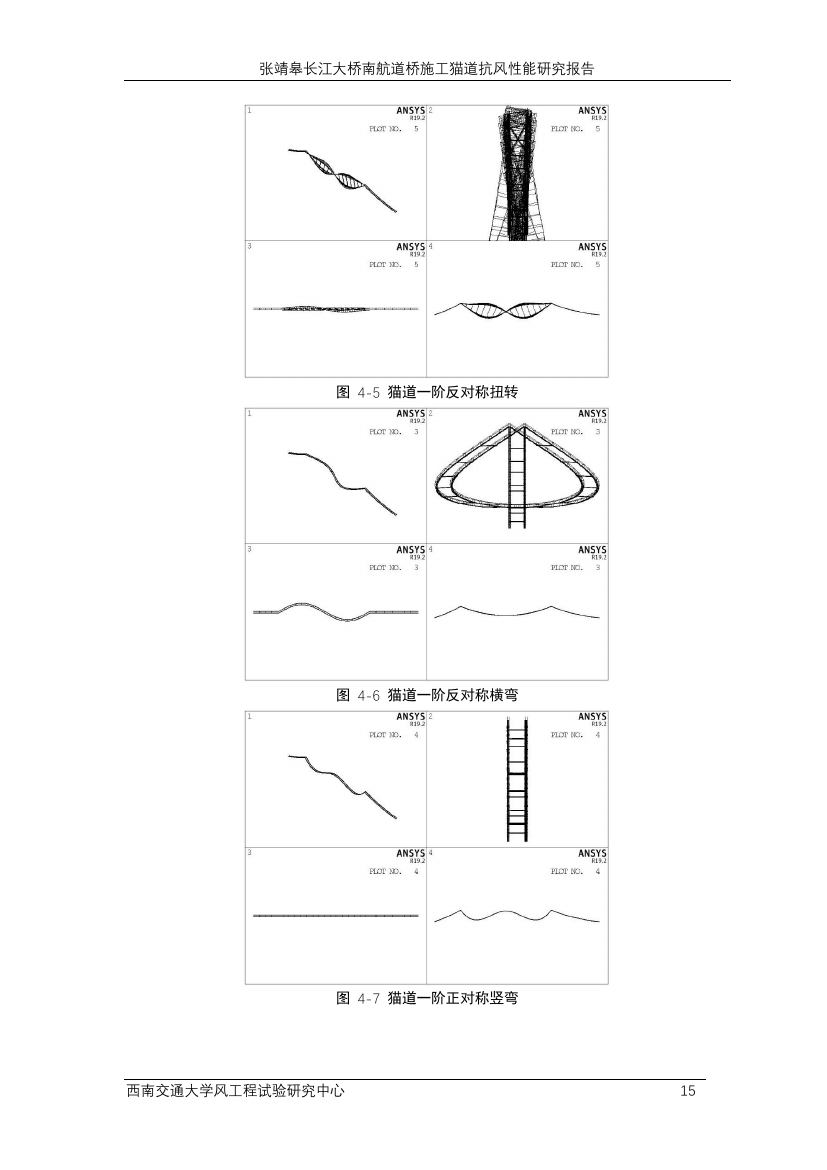
\includegraphics[width=0.48\linewidth]{../inputs/roll_upgrade_sources/drawing_evidence/attachment23_fig4-5_TA1_shape.png}
\caption{左：MD5-17，32 只尼龙滚轮骑在承重索上。右：附件图 4-5 的 TA1——正视双幅反相竖向 X 交叉，与本文系统扭转同一形态。}
\end{figure}

附件 2--3 原文（西南交大风工程中心，32 页，SHA-256 \texttt{d17d4061\ldots}）补充三点：
\begin{enumerate}
  \item 表 4--1 出自其自建 ANSYS 模型，自述为 link10 承重绳 / 门架承重绳 + beam4 大小横梁与门架，扶手系统只均布质量。
  \item 图 4-5 的 TA1 不是某种未知形态，就是双幅反相竖向。同一形态，附件算得 0.0996~Hz，审计装配算得 $\approx0.071$~Hz。
  \item V2 历程（2026-07-12/13）写明：R19.2 源模型完整输入从未取得；历史动力结果已永久删除。\textbf{迄今没有任何模型复现过表 4--1 的 T 行。}
\end{enumerate}

VS2（$-17\%$）在本次升级里几乎不动。它与全部扭转 / 门架通路解耦，指向索系弹性状态（EA / 初张力 / 弹模口径），维持``未定位''。钢丝绳弹模取值差即可产生 $+20\%$ 量级，但这是口径假设，不是已核证来源。

\section{另一条路径：f99-chain-closure 全模型}

用户给出 \url{https://github.com/Hiram-test/model/tree/f99-chain-closure}，要求结合前面结论一起看。这条路径与 ROM 升级独立：它是全尺度 ANSYS（约 $1.09\times10^{5}$ 节点、$1.73\times10^{5}$ 单元），按``销 / 抱箍 / 下压索 / 横通道刚臂''逐枪改连接，每枪对表 4--1 做物理配对（禁止按阶次硬配，禁止把杂交对的第 4 阶标成 TA1）。

\subsection{连接链与表 4--1 的 T 行}

\begin{table}[h]\centering\footnotesize
\begin{tabular}{llrrr}
\toprule
工况 & 改了什么 & TA1 Hz（误差） & TS1 & TS2 \\
\midrule
附件 & —— & 0.0996 & 0.1147 & 0.1571 \\
S10 / C20 & 上销 ROTX、CERIG 保留 & 0.07336 ($-26.4\%$) & 0.10338 & 0.14966 \\
D10 & 32 根物理下压索（总 EA/轴力同 C20） & 0.07337 ($-26.3\%$) & 0.10337 & 0.14964 \\
E10 & 1386 条通道 CERIG ALL$\to$UXYZ & 0.07333 ($-26.4\%$) & 0.10335 & 0.14961 \\
E20 & 通道刚臂$\to$4158 个 COMBIN14，$k=10^{4}$~N/mm & \textbf{0.08445 ($-15.2\%$)} & 0.10607 & 0.15100 \\
\bottomrule
\end{tabular}
\caption{$f99$ 链的 T 行。C20/D10/E10 的 $\Delta f$ 在 $10^{-5}$~Hz 量级；E20 是第一次离开摆式地板。E21（$k=10^{3}$）在该分支快照时仍在求解。}
\end{table}

$f99$ 自己的文字已经把机制写死了：
\begin{itemize}
  \item D10：``反对称扭转刚度不足的根因不在下压索。TA1 与纯张力反对称根 $2f^\ast\approx0.07344\,\mathrm{Hz}$ 重合。''
  \item E10：``ALL$\to$UXYZ 不是 TA1 开关。真正被松开的是门架 ROTX 局部簇（M27/M28 降 $0.78\times10^{-3}$~Hz），四端口相对平动没有进入反对称滚转。''
  \item E20：``第一次把 TA1 从纯张力根 $2f^\ast$ 抬起来。LA--TA 杂交对拆开，TA1 成为干净反对称扭转（shareT$=0.981$）。$k=10^{4}$~N/mm 仍比 v5 $\lambda_1=3.25$~N/mm 硬约 3000 倍。仍禁止封 F00。''
\end{itemize}

这与引理 A 逐字对齐：销、下压索、释放通道转角，全都碰不到系统扭转的摆式地板。全模型和 ROM 用两套完全不同的离散，钉在同一个频率上。

\subsection{E20 抬升是什么，不是什么}

E20 的数值是真的：TA1 从 0.07333 升到 0.08445，$\Delta=+0.01112$~Hz；LS1/VA1/VS1 不动，说明弹簧没有破坏整体横弯 / 竖弯。但它不是图纸连接的客观恢复：
\begin{itemize}
  \item 物理连接是尼龙滚轮骑索 + U 栓抱夹 + 销 / 抱箍，不是三向 $10^{4}$~N/mm 的线弹簧；
  \item 该 $k$ 比他们自己引用的软特征值硬三个数量级，是旋钮，不是出处；
  \item 弹簧在四端口相对平动上做功。滚轮连接在这些方向上并不提供同等储能。把刚体运动学里不该有的相对位移能加进去，就是早先讨论里说的``伪能量''：频率被抬高，来源不是审计部件。
\end{itemize}
ROM 侧的括弧已经预言：只有插入``审计部件不含的相对平动能''才能离开摆式地板。E20 是这个预言的全模型实例。它把 TA1 从 $-26\%$ 收到 $-15\%$，仍到不了 0.0996；再降 $k$（E21）只是沿着同一旋钮滑动，不会把需求值变成来源值。

\begin{figure}[h]\centering
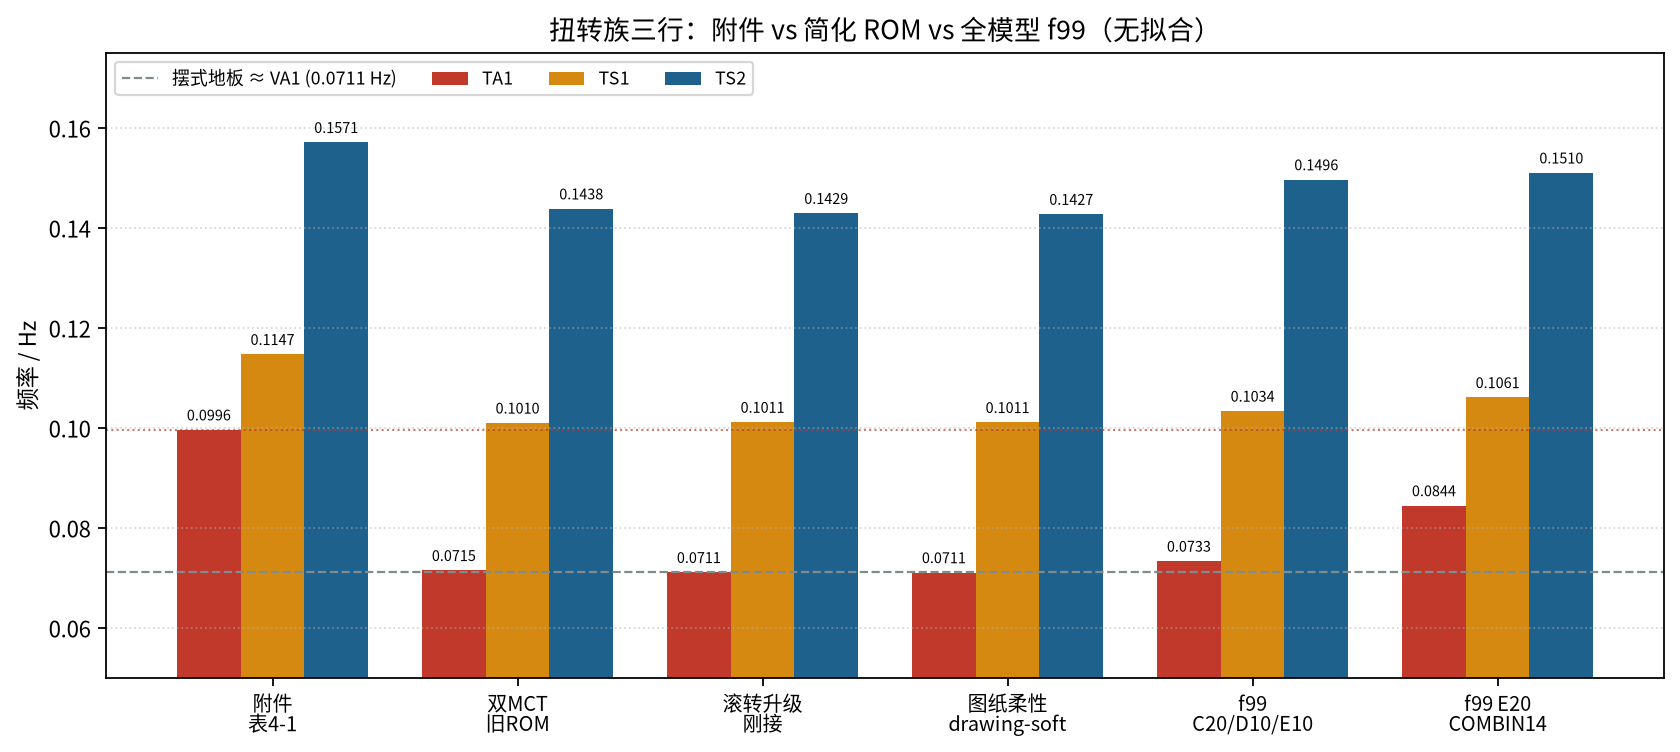
\includegraphics[width=0.98\linewidth]{assets/torsion_family_cross_model.png}
\caption{T 三行跨模型对照。附件是孤立的上沿；ROM 三代与 $f99$ 的 C20/D10/E10 都贴在摆式地板附近；只有 E20 弹簧旋钮把它抬离。}
\end{figure}

\begin{figure}[h]\centering
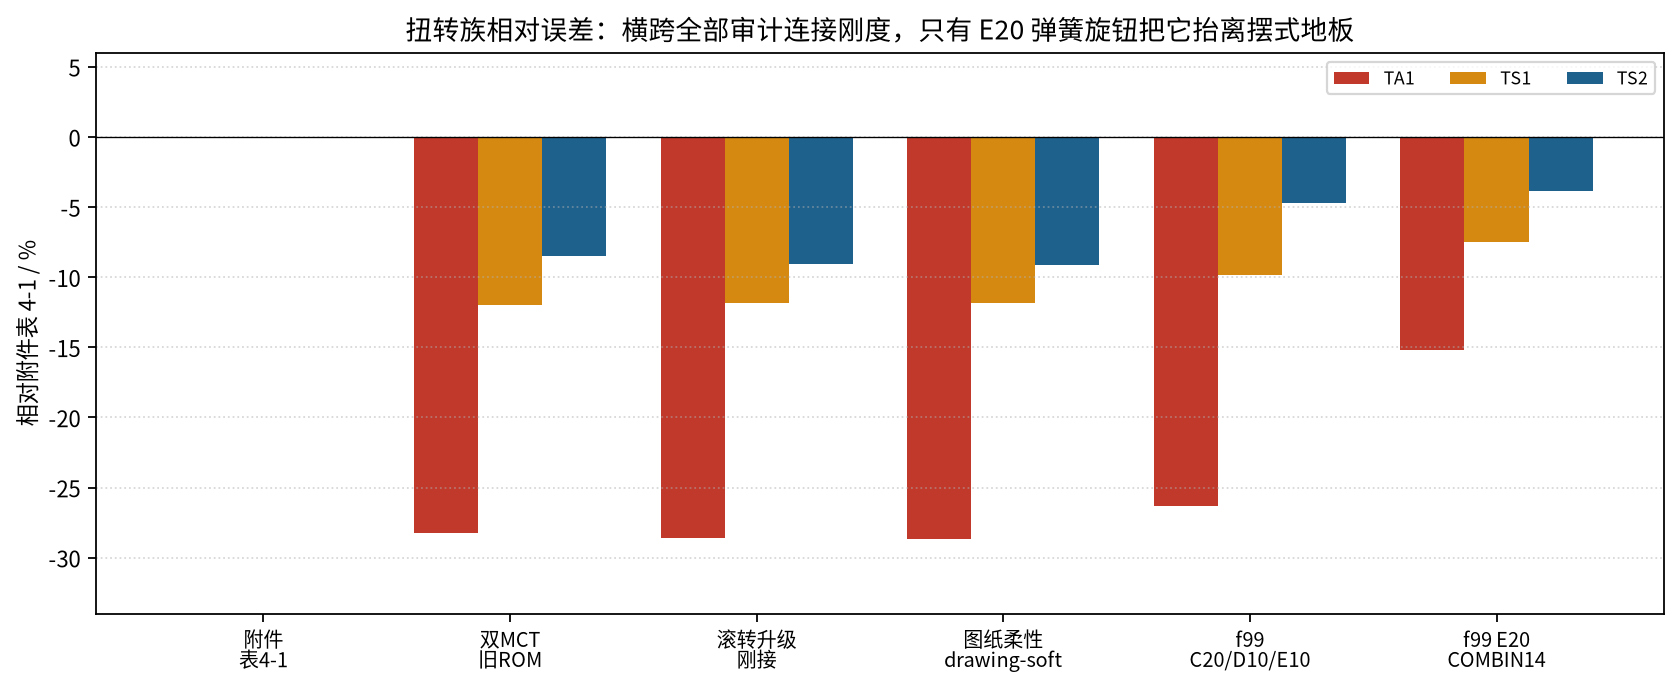
\includegraphics[width=0.98\linewidth]{assets/torsion_family_cross_model_error.png}
\caption{相对附件的误差。刚接 / 柔性 / 全模型铰接链叠在同一条带上；E20 是带外的唯一点，且仍差 $-15\%$。}
\end{figure}

$f99$ 还有一个与 ROM 不同的现象：LA2 被配到 $\approx0.220$~Hz（$+52\%$）。那是全模型里二阶反对称横弯被门架局部 ROTX 簇挤到后面的配对，置信度低，他们自己标了``低置信''。它不改变 T 族结论，只说明两条路径的高阶 L 口径本来就不同，不能混用。

\section{两条路径对照后的定案}

把 ROM 升级和 $f99$ 全模型放在一张桌子上，能一起说的只有这些：

\begin{enumerate}
  \item \textbf{形态一致}。附件图 4-5、ROM 系统扭转、全模型 TA 行，都是双幅反相竖向。争的是同一形态的频率，不是认错了模态。
  \item \textbf{地板一致}。凡是只用审计钢结构 + 索幕 + 图纸级连接（U 栓 / 滚轮 / 销 / 抱箍 / CERIG 或 UXYZ），TA1 都停在 $0.071$--$0.073$~Hz，与 VA1 或 $2f^\ast$ 重合。简化模型和 10 万节点模型给出同一个括弧下沿。
  \item \textbf{刚接与柔性一致}。ROM 的 cerig-rigid 与 drawing-soft、全模型的 C20/D10/E10，横跨全部物理连接刚度，T 族几乎不动。连接细节不是开关。
  \item \textbf{唯有非出处弹簧能离开地板}。E20 的 COMBIN14 是目前唯一把 TA1 抬离 $2f^\ast$ 的算例，而它的 $k$ 不是图纸参数。这强化而不是削弱括弧：离开地板必须引入审计部件没有的相对平动能。
  \item \textbf{举证责任已经转移}。对方单位不会提供 R19.2 源模型——讨论里已经按这个前提处理。在这个前提下，不能再把``我们没复现''默认为``我们的模型错了''。现有证据更支持：附件表 4--1 的 T 行依赖一个未公开、且与图纸连接 / 摆式物理不一致的隐含假设（质量横向分布、连接储能，或索 EA/初张力口径）。VS2 的 $-17\%$ 指向同一类口径问题，但与扭转通路解耦。
\end{enumerate}

一个月没复现出来，不是因为少改了一处销或少加了一根下压索。两条独立路径把这个范围扫完了。

\section{能说什么 / 不能说什么}

\textbf{能说}
\begin{itemize}
  \item 锁定正式配对的十四行数字、T/非 T 分族、半波不作配对依据——这些仍成立。
  \item 双索组 + 双簇端口 + 空间化质量，在结构层面补回了平面化切断的三条通路；主跨非 T 行改善或持平；两类非物理分支被治愈。
  \item 系统扭转钉扎与幅内滚转锁定两条引理，加上图纸柔性端和 $f99$ 全模型链，把 T 族偏差从``未解释的模型误差''变成``审计部件可达域之外''的定量结论。
  \item 附件 TA1 与其自述模型、图纸连接、摆式物理三者联立后，在现有公开输入下不可达。
\end{itemize}

\textbf{不能说}
\begin{itemize}
  \item 不能宣布复现表 4--1（T 族仍 $-28.6/-11.8/-9.0\%$ 或全模型 $-26/-10/-5\%$；VS2 仍 $-17\%$ 或全模型 $+7.5\%$——两条路径的 VS2 符号都对不上附件，更不能互相冒充）。
  \item 不能把反推的 $10^{4}$~N·m/rad/品 或 E20 的 $10^{4}$~N/mm 当作设计事实。
  \item 不能说附件``一定算错了''。没有 R19.2 源模型，只能说它的 T 行与公开图纸和摆式物理不一致；对错属于对方模型的内部问题。
  \item 簇内刚性、H10 代表矩阵复用、等张力分摊、二期质量横向双线表达、全模型 LA2 低置信配对，都是显式近似。
  \item 本文 not\_a\_scientific\_claim。
\end{itemize}

\section{还缺什么，缺了也不该再调}

定案所缺的仍是同一件东西：附件原始 ANSYS 输入（R19.2 源模型）——质量怎么铺、门架 / 横通道怎么连、索 EA 与初张力取哪组数。对方不会给。在这个约束下，继续改销、改下压、改 CERIG 类型、或把弹簧 $k$ 滑向 0.0996，都不会把``需求值''变成``来源值''。

值得另开、且与扭转解耦的，只剩 VS2 的索系弹性口径（弹模 / 张力 / 温度），以及 175 页《图纸汇总-2026.08.05.pdf》若出现与 1225 版不同的通道数量或连接。这两件事都不改变括弧下沿。

\appendix
\section{文件与出处}

\begin{itemize}
  \item 锁定配对：\texttt{catwalk-fem/double-mct-buffeting/modal\_validation/gate\_corrected\_*}
  \item 理论修复代码：\texttt{code/condense\_h10\_cluster\_ports.py}；
        \newline\texttt{code/double\_mct\_roll\_upgraded\_model.py}
  \item 升级结果：\texttt{roll\_upgraded\_results/}，柔性变体 \texttt{roll\_upgraded\_results\_drawing\_soft/}
  \item 推导 PDF：\texttt{report/double\_mct\_torsion\_theory\_fix\_cn.pdf}
  \item 图证：\texttt{inputs/roll\_upgrade\_sources/drawing\_evidence/}
  \item f99 对照：分支 \texttt{f99-chain-closure} 下
        \texttt{ultra\_runs/frequency\_compare\_*.md} 与各工况 \texttt{qa/*table41*}
\end{itemize}

复现升级模型（不重跑 $f99$ ANSYS）：
\begin{verbatim}
python code/condense_h10_cluster_ports.py
python code/double_mct_roll_upgraded_model.py --modes 80
python code/double_mct_roll_upgraded_model.py --modes 80 \
    --passage-mode drawing-soft --output roll_upgraded_results_drawing_soft
\end{verbatim}

\end{document}
